% This is text associated with the open textbook "Open Electromagnetics"
% See immediately below for author, date
% This work is licensed under the Creative Commons Attribution-ShareAlike 4.0 International License. (CC BY-SA 4.0) 
% To view a copy of the license, visit http://creativecommons.org/licenses/by-sa/4.0/

%ORB TITLE Parallel Plate Waveguide: TE Case, Electric Field
%ORB AUTHOR 0        # S.W. Ellingson, Virginia Tech (ellingson@vt.edu)
%ORB DATE 20191202   # yyyymmdd
%ORB ABSTRACT 

\label{m0174_Parallel_Plate_Waveguide_TE_Electric} % <-- Must match name of this file and module directory name.  Don't mess with this!
\index{waveguide!parallel plate|(}
\index{parallel-plate waveguide|see{waveguide}}

In Section~\ref{m0173_Parallel_Plate_Waveguide_Introduction}, the parallel plate waveguide was introduced.
At the end of that section, we described the decomposition of the problem into its TE and TM components.
In this section, we find the electric field component of the TE field in the waveguide.

Figure~\ref{m0174_fParallelPlateWaveguide} shows the problem addressed in this section. 
(Additional details and assumptions are addressed in Section~\ref{m0173_Parallel_Plate_Waveguide_Introduction}.)
%
\begin{figure}[b!] % <--- "[b]" for first figure in section *only*; delete for 2nd and subsequent figures
\begin{center}
\pdftooltip{{  % note double braces
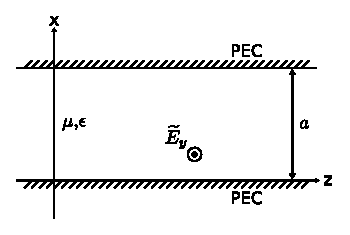
\includegraphics[width=0.8\columnwidth]{modules/m0174_fParallelPlateWaveguide.eps} 
% https://commons.wikimedia.org/wiki/File:TE_component_of_electric_field_in_parallel_plate_waveguide.svg
}}{For a z-x Cartesian coordinate system there are two parallel plates a distance small a apart. The interior region is labeled small mu comma small epsilon and has an electric field out of page labeled capital e tilde subscript small y.}
\end{center}
\centerline{\scriptsize 
\copyright~\hyperref[m0174_fParallelPlateWaveguide_Credit]{C.\ Wang} 
\href{https://creativecommons.org/licenses/by-sa/4.0/}{CC BY-SA 4.0} 
} % \centerline 
\caption{
\label{m0174_fParallelPlateWaveguide}
TE component of the electric field in a parallel plate waveguide.
}
\end{figure}

Since $\widetilde{E}_x=\widetilde{E}_z=0$ for the TE component of the electric field, Equations~\ref{m0173_eEfx2} and \ref{m0173_eEfz2} are irrelevant, leaving only:
%
\begin{equation}
\frac{\partial^2}{\partial x^2}\widetilde{E}_y + \frac{\partial^2}{\partial z^2}\widetilde{E}_y = - \beta^2 \widetilde{E}_y 
\label{m0174_eDE}
\end{equation}
%
The general solution to this partial differential equation is:
%
\begin{flalign}
\widetilde{E}_y =&~~~~~e^{-jk_z z} \left[ A e^{-jk_x x} + B e^{+jk_x x} \right] \nonumber \\
                 &+e^{+jk_z z} \left[ C e^{-jk_x x} + D e^{+jk_x x} \right] 
\label{m0174_eGS}
\end{flalign}
%
where 
$A$, $B$, $C$, and $D$ are complex-valued constants and 
$k_x$ and $k_z$ are real-valued constants.
We have assigned variable names to these constants with advance knowledge of their physical interpretation; however, at this moment they remain simply unknown constants whose values must be determined by enforcement of boundary conditions.

Note that Equation~\ref{m0174_eGS} consists of two terms.
The first term includes the factor $e^{-jk_z z}$, indicating a wave propagating in the $+\hat{\bf z}$ direction, and
the second term includes the factor $e^{+jk_z z}$, indicating a wave propagating in the $-\hat{\bf z}$ direction.
If we impose the restriction that sources exist only on the left ($z<0$) side of Figure~\ref{m0174_fParallelPlateWaveguide}, and that there be no structure capable of wave scattering (in particular, reflection) on the right ($z>0$) side of Figure~\ref{m0174_fParallelPlateWaveguide}, then there can be no wave components propagating in the $-\hat{\bf z}$ direction.  In this case, $C=D=0$ and Equation~\ref{m0174_eGS} simplifies to:
%
\begin{equation}
\widetilde{E}_y = e^{-jk_z z} \left[ A e^{-jk_x x} + B e^{+jk_x x} \right] 
\label{m0174_eGS2}
\end{equation}

Before proceeding, let's make sure that Equation~\ref{m0174_eGS2} is actually a solution to Equation~\ref{m0174_eDE}.
As we shall see in a moment, performing this check will reveal some additional useful information.
First, note:
%
\begin{equation}
\frac{\partial \widetilde{E}_y}{\partial x} = e^{-jk_z z} \left[-A e^{-jk_x x} + B e^{+jk_x x} \right]\left(jk_x\right) 
\end{equation}
%
So:
%
\begin{equation}
\frac{\partial^2 \widetilde{E}_y}{\partial x^2} = e^{-jk_z z} \left[ A e^{-jk_x x} + B e^{+jk_x x} \right]\left(-k_x^2\right)
\end{equation}
%
Comparing this to Equation~\ref{m0174_eGS2}, we observe the remarkable fact that
%
\begin{equation}
\frac{\partial^2 \widetilde{E}_y}{\partial x^2} = -k_x^2 \widetilde{E}_y
\end{equation}
%
Similarly, note:
%
\begin{equation}
\frac{\partial \widetilde{E}_y}{\partial z}     = e^{-jk_z z} \left[ A e^{-jk_x x} + B e^{+jk_x x} \right]\left(-jk_z\right) 
\end{equation}
%
So:
%
\begin{flalign}
\frac{\partial^2 \widetilde{E}_y}{\partial z^2} &= e^{-jk_z z} \left[ A e^{-jk_x x} + B e^{+jk_x x} \right]\left(-k_z^2\right) \nonumber \\
                                                &= -k_z^2 \widetilde{E}_y
\end{flalign}
%
Now summing these results:
%
\begin{equation}
\frac{\partial^2 \widetilde{E}_y}{\partial x^2} + \frac{\partial^2 \widetilde{E}_y}{\partial z^2} = -\left( k_x^2 + k_z^2 \right) \widetilde{E}_y
\label{m0174_eDE2}
\end{equation}
%
Comparing Equation~\ref{m0174_eDE2} to Equation~\ref{m0174_eDE}, we conclude that Equation~\ref{m0174_eGS2} is indeed a solution to Equation~\ref{m0174_eDE}, but only if:
%
\begin{equation}
\beta^2 = k_x^2 + k_z^2
\label{m0174_eBeta}
\end{equation}
%
This confirms that $k_x$ and $k_z$ are in fact the components of the propagation vector
%
\begin{equation}
{\bf k} \triangleq \beta\hat{\bf k} = \hat{\bf x}k_x + \hat{\bf y}k_y + \hat{\bf z}k_z
\end{equation}
%
where $\hat{\bf k}$ is the unit vector pointing in the direction of propagation, and $k_y=0$ in this particular problem. 

The solution has now been reduced to finding the constants $A$, $B$, and either $k_x$ or $k_z$.
This is accomplished by enforcing the relevant boundary conditions.
In general, the component of $\widetilde{\bf E}$ that is tangent to a perfectly-conducting surface is zero.
Applied to the present problem, this means 
$\widetilde{E}_y = 0$ at $x=0$ and
$\widetilde{E}_y = 0$ at $x=a$.
Referring to Equation~\ref{m0174_eGS2}, the boundary condition at $x=0$ means
%
\begin{equation}
e^{-jk_z z} \left[ A \cdot 1 + B \cdot 1 \right] = 0
\end{equation} 
%
The factor $e^{-jk_z z}$ cannot be zero; therefore, $A+B=0$.
Since $B=-A$, we may rewrite Equation~\ref{m0174_eGS2} as follows:
%
\begin{equation}
\widetilde{E}_y = e^{-jk_z z} B \left[ e^{+jk_x x} - e^{-jk_x x} \right] 
\end{equation}
%
This expression is simplified using a trigonometric identity:
%
\begin{equation}
\frac{1}{2j}\left[ e^{+jk_x x} - e^{-jk_x x} \right] = \sin{k_x x} 
\end{equation} 
%
Let us now make the definition $E_{y0}\triangleq j2B$.  Then:
%
\begin{equation}
\widetilde{E}_y = E_{y0} e^{-jk_z z} \sin k_x x
\label{m0174_eGS3}
\end{equation}
%
Now applying the boundary condition at $x=a$:
%
\begin{equation}
E_{y0} e^{-jk_z z} \sin k_x a  = 0
\end{equation} 
%
The factor $e^{-jk_z z}$ cannot be zero, and $E_{y0}=0$ yields only trivial solutions; therefore: 
%
\begin{equation}
\sin{k_x a} = 0
\end{equation} 
%
This in turn requires that
%
\begin{equation}
k_x a = m \pi 
\label{m0174_ekxa}
\end{equation}
%
where $m$ is an integer.
Note that $m=0$ is not of interest since this yields $k_x=0$, which according to Equation~\ref{m0174_eGS3} yields the trivial solution $\widetilde{E}_y=0$.
Also each integer value of $m$ that is less than zero is excluded because the associated solution is different from the solution for the corresponding positive value of $m$ in sign only, which can be absorbed in the arbitrary constant $E_{y0}$.

At this point we have uncovered a family of solutions given by Equation~\ref{m0174_eGS3} and Equation~\ref{m0174_ekxa} with $m=1,2,...$.
Each solution associated with a particular value of $m$ is referred to as a \emph{mode}, which (via Equation~\ref{m0174_ekxa}) has a particular value of $k_x$.
\index{mode}
The value of $k_z$ for mode~$m$ is obtained using Equation~\ref{m0174_eBeta} as follows:
%
\begin{flalign}
k_z &= \sqrt{\beta^2-k_x^2} \nonumber \\
    & =\sqrt{\beta^2-\left(\frac{m\pi}{a}\right)^2}
\end{flalign}
%
Since $k_z$ is specified to be real-valued, we require:
%
\begin{equation}
\beta^2-\left(\frac{m\pi}{a}\right)^2 > 0
\end{equation}
%
This constrains $\beta$; specifically:
%
\begin{equation}
\beta > \frac{m\pi}{a}
\end{equation}
%
Recall that $\beta=\omega\sqrt{\mu\epsilon}$ and $\omega=2\pi f$ where $f$ is frequency.
Solving for $f$, we find:
%
\begin{equation}
f > \frac{m}{2a\sqrt{\mu\epsilon}}
\end{equation}
%
Therefore, each mode exists only above a certain frequency, which is different for each mode. 
This \emph{cutoff frequency}
\index{cutoff frequency}
$f_c$ for mode $m$ is given by 
 %
\begin{equation}
\boxed{
f_c^{(m)} \triangleq \frac{m}{2a\sqrt{\mu\epsilon}}
}
\label{m0174_efcm}
\end{equation}
%
At frequencies below the cutoff frequency for mode $m$, modes $1$ through $m-1$ exhibit imaginary-valued $k_z$.
The propagation constant must have a real-valued component in order to propagate; therefore, these modes do not propagate and may be ignored. 

Let us now summarize the solution.
For the scenario depicted in Figure~\ref{m0174_fParallelPlateWaveguide}, the electric field component of the TE solution is given by:
%
\begin{equation}
\boxed{
\hat{\bf y}\widetilde{E}_y = \hat{\bf y}\sum_{m=1}^{\infty} \widetilde{E}_y^{(m)}
}
\label{m0174_eEysum}
\end{equation}
%
where
%
\begin{equation}
\boxed{
\widetilde{E}_y^{(m)} \triangleq \begin{cases}
                                   0,                             & f<f_c^{(m)} \\
                                   E_{y0}^{(m)} e^{-jk_z^{(m)} z} \sin k_x^{(m)} x, & f\ge f_c^{(m)} 
                                 \end{cases}
}
\end{equation}
%
where $m$ enumerates modes ($m=1,2,...$),
%
\begin{equation}
\boxed{
k_z^{(m)} \triangleq \sqrt{\beta^2-\left[k_x^{(m)}\right]^2}
}
\end{equation}
%
and
%
\begin{equation}
\boxed{
k_x^{(m)} \triangleq m\pi/a 
}
\label{m0174_ekxma}
\end{equation}
%
Finally, $E_{y0}^{(m)}$ is a complex-valued constant that depends on sources or boundary conditions to the left of the region of interest.
%
%%%%%%%%%%%%%%%%%%%%%%%%%%%%%%%%%%%%%%%%%%%%%%%
%ORB HIGHLIGHT
\begin{mdframed}[backgroundcolor=yellow!20,nobreak=true] 
For the scenario depicted in Figure~\ref{m0174_fParallelPlateWaveguide}, the electric field component of the TE solution is given by Equation~\ref{m0174_eEysum} with modal components determined as indicated by Equations~\ref{m0174_efcm}--\ref{m0174_ekxma}.  This solution presumes all sources lie to the left of the region of interest, and no scattering occurs to the right of the region of interest.
\end{mdframed}
%%%%%%%%%%%%%%%%%%%%%%%%%%%%%%%%%%%%%%%%%%%%%%%

To better understand this result, let us examine the lowest-order mode, $m=1$.
For this mode $f_c^{(1)}=1/2a\sqrt{\mu\epsilon}$, so this mode can exist if $f>1/2a\sqrt{\mu\epsilon}$.
Also $k_x^{(1)} = \pi/a$, so 
%
\begin{equation}
k_z^{(1)} = \sqrt{\beta^2-\left(\frac{\pi}{a}\right)^2}
\label{m0174_ekz1}
\end{equation}
%
Subsequently,
%
\begin{equation}
\widetilde{E}_y^{(1)} = E_{y0}^{(1)} e^{-jk_z^{(1)} z} \sin \frac{\pi x}{a} 
\end{equation}
%
Note that this mode has the form of a plane wave.
The plane wave propagates in the $+\hat{\bf z}$ direction with phase propagation constant $k_z^{(1)}$.
Also, we observe that the apparent plane wave is non-uniform, exhibiting magnitude proportional to $\sin \pi x/a$ within the waveguide.
This is shown in Figure~\ref{m0174_fParallelPlateWaveguide-TEmodes} (left image).
%
\begin{figure} % <--- "[b]" for first figure in section *only*; delete for 2nd and subsequent figures
\begin{center}
\pdftooltip{{  % note double braces
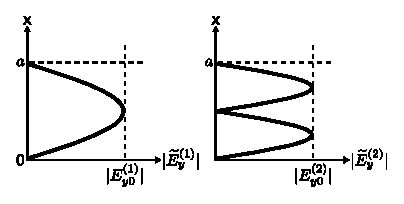
\includegraphics[width=\columnwidth]{modules/m0174_fParallelPlateWaveguide-TEmodes.eps} 
% https://commons.wikimedia.org/wiki/File:Magnitude_of_the_two_lowest-order_TE_modes_in_parallel_plate_waveguide.svg
}}{Left: Magnitude of the m equals 1 mode has the form of one half-period of sine, with zeros at the waveguide plates.  Right: Magnitude of the m equals 2 mode has the form of two half-periods of sine, with zeros at the waveguide plates and the center of the waveguide.}
\end{center}
\centerline{\scriptsize 
\copyright~\hyperref[m0174_fParallelPlateWaveguide-TEmodes_Credit]{C.\ Wang} 
\href{https://creativecommons.org/licenses/by-sa/4.0/}{CC BY-SA 4.0} 
} % \centerline 
\caption{
\label{m0174_fParallelPlateWaveguide-TEmodes}
Magnitude of the two lowest-order TE modes in a parallel plate waveguide. \emph{Left:} $m=1$, \emph{Right:} $m=2$.
}
\end{figure}
%
In particular, we observe that the magnitude of the wave is zero at the perfectly-conducting surfaces -- as is necessary to satisfy the boundary conditions -- and is maximum in the center of the waveguide.

Now let us examine the $m=2$ mode.
For this mode, $f_c^{(2)}=1/a\sqrt{\mu\epsilon}$, so this mode can exist if $f>1/a\sqrt{\mu\epsilon}$.
This frequency is higher than $f_c^{(1)}$, so the $m=1$ mode can exist at any frequency at which the $m=2$ mode exists.
Also $k_x^{(2)} = 2\pi/a$, so 
%
\begin{equation}
k_z^{(2)} = \sqrt{\beta^2-\left(\frac{2\pi}{a}\right)^2}
\label{m0174_ekz2}
\end{equation}
%
Subsequently,
%
\begin{equation}
\widetilde{E}_y^{(2)} = E_{y0}^{(2)} e^{-jk_z^{(2)} z} \sin \frac{2\pi x}{a} 
\end{equation}
%
In this case, the apparent plane wave propagates in the $+\hat{\bf z}$ direction with phase propagation constant $k_z^{(2)}$, which is less than $k_z^{(1)}$.
For $m=2$, we find magnitude is proportional to $\sin 2\pi x/a$ within the waveguide (Figure~\ref{m0174_fParallelPlateWaveguide-TEmodes}, right image).
As in the $m=1$ case, we observe that the magnitude of the wave is zero at the PEC surfaces; however, for $m=2$, there are \emph{two} maxima with respect to $x$, and the magnitude in the center of the waveguide is zero.

This pattern continues for higher-order modes.
In particular, each successive mode exhibits higher cutoff frequency, smaller propagation constant, and increasing integer number of sinusoidal half-periods in magnitude.  

%%%%%%%%%%%%%%%%%%%%%%%%%%%%%%%%%%%%%%%%%%%%%%%
%ORB EXAMPLE
~\\ \begin{example} 
\begin{mdframed}[backgroundcolor=brown!20,linecolor=brown!20]\raggedright
Single-mode TE propagation in a parallel plate waveguide. 
\\~\\
Consider an air-filled parallel plate waveguide consisting of plates separated by $1$~cm.
Determine the frequency range for which one (and only one) propagating TE mode is assured.

\noindent
{\bf Solution.}
Single-mode TE propagation is assured by limiting frequency $f$ to greater than the cutoff frequency for $m=1$, but lower than the cutoff frequency for $m=2$.
(Any frequency higher than the cutoff frequency for $m=2$ allows at least 2 modes to exist.)
Calculating the applicable cutoff frequencies, we find:
%
\begin{flalign}
f_c^{(1)} &= \frac{1}{2a\sqrt{\mu_0\epsilon_0}} \cong 15.0~\mbox{GHz} \\
f_c^{(2)} &= \frac{2}{2a\sqrt{\mu_0\epsilon_0}} \cong 30.0~\mbox{GHz} 
\end{flalign}
%
Therefore, \underline{15.0~GHz $\le f \le$ 30.0~GHz}.
\end{mdframed}
% note figures will need to go between "\end{mdframed}" and "\end{example}"
\end{example}
%%%%%%%%%%%%%%%%%%%%%%%%%%%%%%%%%%%%%%%%%%%%%%%

Finally, let us consider the phase velocity $v_p$ within the waveguide.
For lowest-order mode $m=1$, this is 
%
\begin{equation}
v_p = \frac{\omega}{k_z^{(1)}} = \frac{\omega}{\sqrt{\omega^2\mu\epsilon-\left(\frac{\pi}{a}\right)^2}}
\label{m0174_evp}
\end{equation}
%
Recall that the speed of an electromagnetic wave in unbounded space (i.e., not in a waveguide) is $1/\sqrt{\mu\epsilon}$. 
For example, the speed of light in free space is $1/\sqrt{\mu_0\epsilon_0}=c$.  
However, the phase velocity indicated by Equation~\ref{m0174_evp} is \emph{greater} than $1/\sqrt{\mu\epsilon}$; e.g., faster than light would travel in the same material (presuming it were transparent).
At first glance, this may seem to be impossible.
However, recall that \emph{information} travels at the group velocity $v_g$, 
\index{group velocity}
and not necessarily the phase velocity. 
(See Section~\ref{m0176_Phase_and_Group_Velocity} for a refresher.)
Although we shall not demonstrate this here, the group velocity in the parallel plate waveguide is always \emph{less} than $1/\sqrt{\mu\epsilon}$, so no physical laws are broken, and signals travel somewhat slower than the speed of light, as they do in any other structure used to convey signals.

Also remarkable is that the speed of propagation is different for each mode.  In fact, we find that the phase velocity increases and the group velocity decreases as $m$ increases.  This phenomenon is known as \emph{dispersion},
\index{dispersion}
and sometimes specifically as \emph{mode dispersion} or
\emph{modal dispersion}.
%\index{mode (modal) dispersion}

\index{waveguide!parallel plate|)}


